\documentclass[a4paper]{scrartcl}

\usepackage{enumitem}
\usepackage[colorlinks]{hyperref}
\usepackage{graphicx}
\usepackage{caption}
\usepackage{subcaption}

\usepackage{multicol}
% \usepackage{savetrees}

\usepackage{listings}
\usepackage{listings-golang}
\lstset{ % add your own preferences
    frame=single,
    basicstyle=\footnotesize,
    keywordstyle=\color{red},
    numbers=left,
    numbersep=5pt,
    showstringspaces=false,
    stringstyle=\color{blue},
    tabsize=4,
    language=Golang % this is it !
}
% Template for homework assignment @ FI muni

% Homework setup
\newcommand{\authorName}{Mgr.~Vladim\'{i}r Sedl\'{a}\v{c}ek, Bc.~Jan~Kvapil, Bc.~Ondřej Kr\v{c}ma}
\newcommand{\courseID}{\texttt{PV204}}
\newcommand{\homeworkID}{\texttt{Report about RSA/ECDSA timing analysis}}

\usepackage{amsthm}
\usepackage{fancyhdr}
\pagestyle{fancy}

% Create a nice header
\fancyhead[L]{\courseID:\homeworkID\\\authorName}
% \fancyhead[C]{\authorName}
\fancyhead[R]{\today}
\renewcommand{\headrulewidth}{0.4pt}

\subtitle{}

\usepackage{titlesec}
\titleformat*{\section}{\large\bfseries}
\begin{document}

% \maketitle

\section{Useful links}
Link to the source code on Github: \url{https://github.com/quapka/go-analysis/}.\\
Link to Google Drive folder with graphs: \url{https://drive.google.com/drive/u/0/folders/1_JAimTs1b7T1Q2X1K-F91Tj63uSdiXed}.
%Add call graph!

\section{Selecting the functions}
After seeing the call graphs (you can use \verb+xdot+ to view them, check \url{https://drive.google.com/drive/u/0/folders/1OQRRlH1eYil-RmBKizMd_bJSGRPLPrs_}) fo RSA decryption/signing and ECDSA, we decided to pick the following functions for further analysis:
\\ECC: ScalarBaseMult, ScalarMult, Add, Double, CombinedMult, Inverse, IsOnCurve.
\\RSA: EncryptPKCS1v15, DecryptPKCS1v15.

All of them seemed either relevant or easy to measure (at least at the first glance), even though we discovered many dependencies between them later. Also, in the ECC case, we decided to fix the curve NIST P-256 for all the functions (as this was the curve we used in the first part of the project). Some of the less interesting functions were left out from the report in the interest of brevity.

\section{ScalarBaseMult}
Commentary: This function computes a scalar multiple of the generator point of the parent curve. In fact, it just calls ScalarMult with the generator point of the curve as input (but it still make sense to measure both of them and observe whether there are any significant differences).
\\Inputs: 1) 1000 random scalars, 2) scalars with weights from 0 to 255 (10 scalars for each weight, 2550), see graph \ref{fig:generic_ScalarBaseMult}.
% \\Graphs:
\\Conclusion: The graphs show a clear trend of time dependency of on the Hamming weight of the scalar. And indeed, digging into the code revealed that this function basically performs only the classical Double-and-Add algorithm (combined with conversions to and from Jacobian coordinates), where both Add and Double are discussed below. This seems quite surprising (considering that Go also implements modern ECC such as Curve25519 with the Montgomery ladder), but can probably be explained by the fact that this is only a general scalar multiplication function and might only be used for testing purposes.

\begin{figure}
    \centering
  \includegraphics[width=0.4\linewidth]{../timers/src/elliptic_ScalarBaseMult/elliptic_ScalarBaseMult_data_weights-medians.png}
  \caption{ScalarBaseMult: increasing weight of the scalar suggests increase of the time needed for the multiplication.}
  \label{fig:generic_ScalarBaseMult}
\end{figure}

\section{ScalarMult}
Commentary: This is the same as ScalarBaseMult, only the multiplied point can be arbitrary (with the exception of the neutral element).
\\Inputs: 1) Points with x coordinate of weights from 0 to 255 (10 points for each weight) and random scalars, 2) random points and scalars with weights from 0 to 255 (10 scalars for each weight). The graph is is quite similar to \ref{fig:generic_ScalarBaseMult}.%, see graph \ref{fig:generic_ScalarMult}).
\\Conclusion: Using other points than the generator one does not seem to significantly affect the graphs, thus the conclusion is the same as for ScalarBaseMult.

\section{P256 ScalarBaseMult}
Commentary: Go language has multiple implementations of ScalarBaseMult -- the generic one seen above, but also ones specially tailored for a given curve like this one, which uses the sliding window method (highly optimized and with some extra protection). And indeed, the trend seen in the previous case is not present here. The visible \textit{peaks} in the graph \ref{fig:p256_ScalarBaseMult} might be due to another process interrupting the computation -- to get more insight we'd need to repeat the computations or perform them on another machine.
\\Inputs: 1) 1000 random scalars, 2) scalars with weights from 0 to 255 (10 scalars for each weight, 2550), see graph \ref{fig:p256_ScalarBaseMult}.
\\Conclusion: It does not seem probable that this function would leak any secret data based on our measurements.

\begin{figure}
    \centering
  \includegraphics[width=0.4\linewidth]{../timers/src/data/data_p256_ScalarBaseMult_random_timing-means.png}
  \caption{P256 ScalarBaseMult: increasing the weight of the scalar does not suggest the increase of the time needed for the multiplication.}
  \label{fig:p256_ScalarBaseMult}
\end{figure}

% \begin{figure}
%     \centering
%   \includegraphics[width=0.4\linewidth]{../timers/src/elliptic_ScalarMult/elliptic_ScalarMult_data_scalar-medians.png}
%   \caption{ScalerMult: increasing weight of the scalar suggests increase of the time needed for the multiplication.}
%   \label{fig:generic_ScalarMult}
% \end{figure}

\section{Add}
Commentary: This function adds two points on the curve, using a conversion to Jacobian coordinates first. The code references the formulas at \url{https://hyperelliptic.org/EFD/g1p/auto-shortw-jacobian-3.html#addition-add-2007-bl}. Note that even though these do not contain any branching, this is not true for the the code, which first checks whether any of points is the neutral element and also later checks whether some intermediate results are negative (and if so, adds the prime $p$ to them).
\\Inputs: Points with x coordinate of weights from 0 to 255 (1 point-point for each weight-weight).
\\Conclusion: Probably no real leak, but the heatmap (see the file \verb+elliptic_Add_heatmap.pdf+) shows \textit{some} dependence on the columns and not on the rows, which is a little surprising (but might be explained by the fact that the formulas used do not use the points symetrically).

\iffalse
\section{Double}
Commentary: This function doubles a point on the curve, using a conversion to Jacobian coordinates first. The code references the formulas at \url{https://hyperelliptic.org/EFD/g1p/auto-shortw-jacobian-3.html#doubling-dbl-2001-b}. The remarks about branching in the Add function remain valid here.
\\Inputs: Points with x coordinate of weights from 0 to 255 (100 points for each weight).
\\Graphs:
\\Conclusion:


\section{CombineMult}
Commentary: This function computes a bilinear combination of the generator point and another given point (useful for ECDSA verification). However, it is just a naive combination of adding together the results of ScalarBaseMult and ScalarMult, so it does not make much sense to analyze it, as we already covered all of these separately.

\section{Inverse}
Commentary:
\\Inputs: 1) 10000 random scalars. 2) Scalars with weights from 0 to 255 (1000 scalars for each weight).
\\Graphs:
\\Conclusion:

\section{IsOnCurve}
Commentary: This function checks whether the given point is on the parent curve.
\\Inputs: Points with x coordinate of weights from 0 to 255 (100 points for each weight).
\\Graphs:
\\Conclusion: We did not expect anything surprising here, as the function is quite straightforward, but we have no explanation of the strangely low times for the first few inputs.
\fi

%Is it worth mentioning this?
\section{DecryptPKCS1v15}
Inputs: Plaintexts with weights from 0 to 1900 (10 plaintexts for each weight), random keys and constant byte generator (generating constantly some byte from 10 to 99).
\\Conclusion: Even though there are  few values (see graph \ref{fig:DecryptPKCS1v15}) that are not that uniform we can hardly infer a potential leak.

\begin{figure}
    \centering
  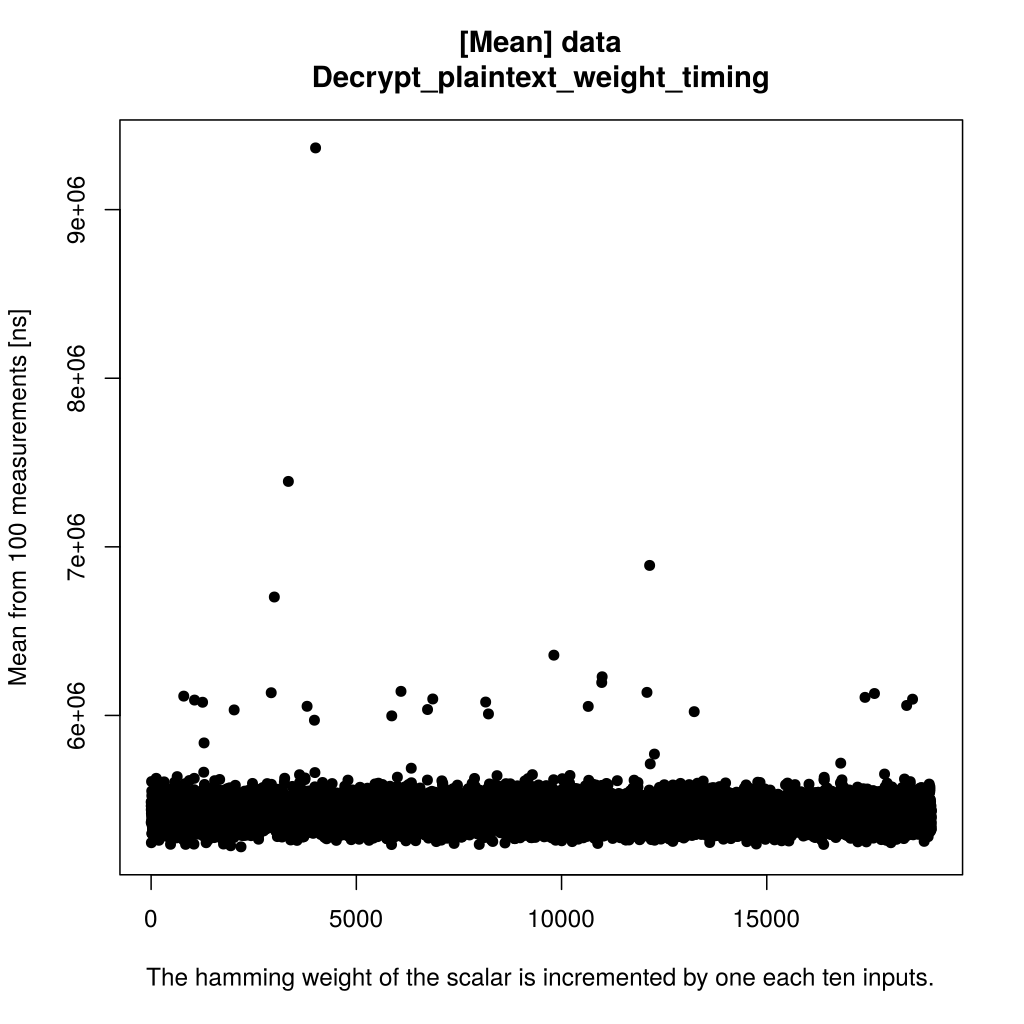
\includegraphics[width=0.4\linewidth]{data_Decrypt_plaintext_weight_timing-means.png}
  \caption{DecryptPKCS1v15}
  \label{fig:DecryptPKCS1v15}
\end{figure}

\iffalse
\section{DecryptPKCS1v15}
Commentary: Same as EncryptPKCS1v15 except plaintexts are replaced with corresponding encrypted plaintexts.
\\Inputs:
\\Graphs:
\\Conclusion:

\begin{figure}
    \centering
  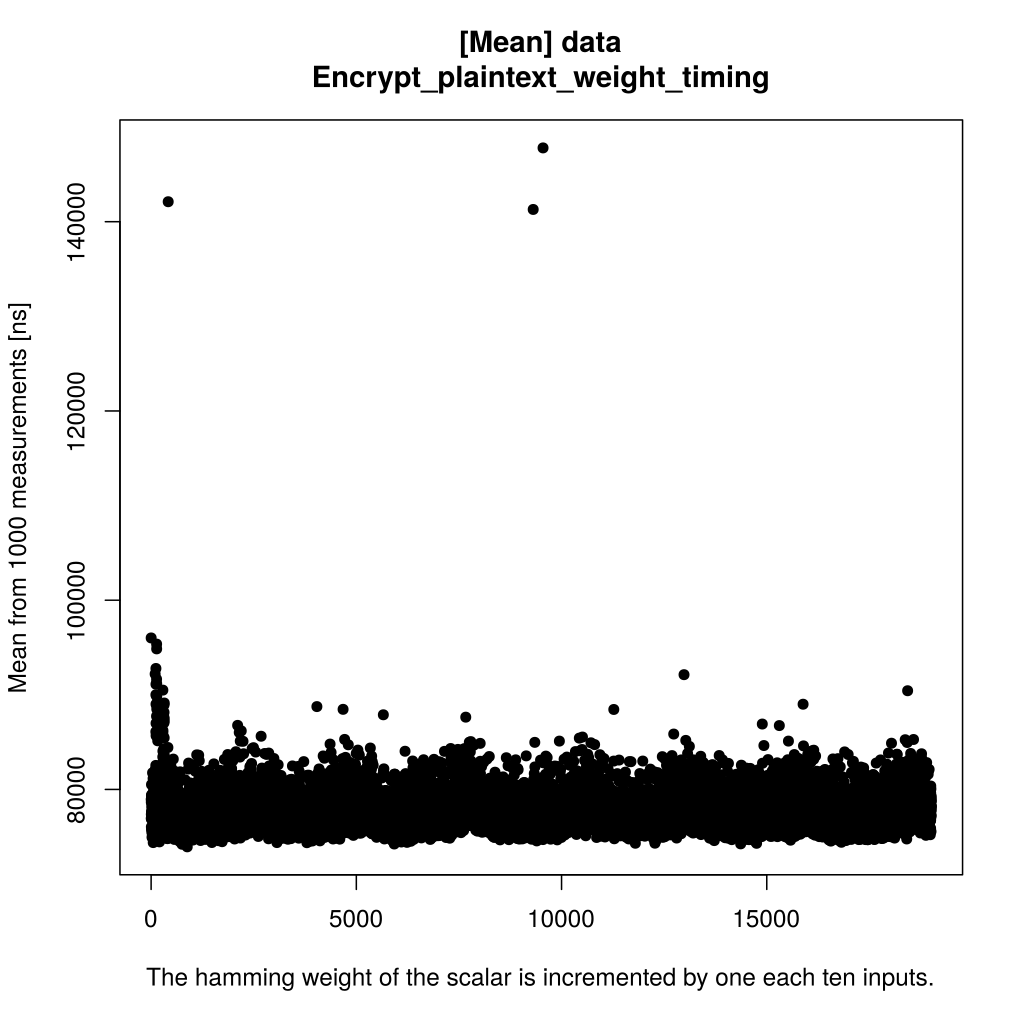
\includegraphics[width=0.4\linewidth]{data_Encrypt_plaintext_weight_timing-means.png}
  \caption{DecryptPKCS1v15}
  \label{fig:DecryptPKCS1v15}
\end{figure}
\fi

\section{Timing the function calls}

We timed the functions in the same way as for previous part of the project:
\begin{lstlisting}[language=golang]
start := time.Now()
_, _ = p256.Params().Add(x1, y1, x2, y2) // measuring Add function
end := time.Now()
elapsed := end.Sub(start)
t1 := elapsed.Nanoseconds()
\end{lstlisting}
%Add some similar details?
%All the keys were generated on the same machine. Generating the RSA 2048 keys took the longest, which was around hour and a half. See Appendix A. for more specification about the machine (all the keys were generated at the same time on specific thread).

\section{Generating graphs}
%Add some similar details?
The graphs were generated using R language. Since we repeated the measurements multiple times (up to 1000 measurements for the same inputs), we then removed potential outliers using the \verb+boxplot+ function. We have reduced the multiple measurements by calculating the mean and median values to get the trend of the measurements rather than individual values.

% \iffalse
% To generate the graphs we wrote a Python3 script using Pandas module. We
% focused on histograms and generation time heatmaps of most and least
% significant bytes of the private keys.
% \\\\
% Most of the graphs show expected distributions. However, histogram of least
% significant byte of $y$ in ECDSA keys shows increased occurrence of bytes \verb+0x00+ to
% \verb+0x0f+. Histogram of MSB of $y$ in ECDSA, on the other hand, shows decreased
% occurrence of bytes \verb+0x00+ to \verb+0x0f+.
% \\\\
% Some graphs didn’t render properly. In most cases this was just a visual
% impairment, however histogram of MSB of $x$ in ECDSA shows first 16 bytes and every
% byte which is multiple of 16 missing. Quick script checking which MSB values
% are actually in the data showed just the first 16 bytes missing. We’re not sure
% yet if the graph is rendered correctly or not.
% \\\\
% Overall, generating graphs in python takes a lot of time and experience with
% the modules, so it might have been better to generate the graphs quickly in
% R (needless to say, we have not got much experience with that either).
% \fi

\section{Summary}
The most interesting result we discovered is definitely the use of the Double-and-Add algorithm in the ScalarBaseMult function, which leaks the Hamming weight of the (potentially secret) scalar. However, this could prove to be an issue only if this function was used in real applications, which does not seem to be the case, as each curve has its own optimized and protected version of scalar multiplication. We did not find any conclusive evidence of weaknesses for the other functions.

% As this function is crucial for almost all ECC schemes, this vulnerability could prove crucial unless some other countermeasures are implemented, as an attacker could quite easily learn the Hamming weight of the secret scalar (and possibly recover it completely). If we do not find any protection against such an attack, we will try to contact the developers.

%Some of the graphs were definitely interesting and it seems worth to do further investigation. Unfortunately, we had troubles to find big enough time windows to get together and do more detailed analysis of the results.


\section{Appendix A. Hardware specifications}
The functions \verb+Add+, \verb+Double+, \verb+ScalarBaseMult+, \verb+ScalarMult+ were measured on the following machine:
\begin{lstlisting}[caption=Hardware specifications of the machine A, captionpos=b]
Model name:          Intel(R) Core(TM) i5-8250U CPU @ 1.60GHz
CPU MHz:             1561.080
CPU max MHz:         3400,0000
CPU min MHz:         400,0000
RAM:                 \~8GB
OS: Ubuntu           18.10
\end{lstlisting}

The rest of the functions on this machine:
\begin{lstlisting}[caption=Hardware specifications of the machine B, captionpos=b]
Model name:          4 core Intel(R) Core(TM) i7-5500U CPU @ 2.40GHz
RAM:                 \~8GB
OS: Ubuntu           Ubuntu 16.04.2
\end{lstlisting}
\end{document}
